\documentclass[12pt]{article}
\usepackage[margin=1in]{geometry}
\usepackage{fancyhdr}
\usepackage{graphicx}
\usepackage{datetime}
\usepackage{float}
\usepackage{amsmath}

\pagestyle{fancy}
\fancyhf{}
\rhead{Brent Myers \\ Econ 5253 \\ 03-23-26}
\renewcommand{\headrulewidth}{0pt}
\setlength{\headheight}{50pt}
\setlength{\headsep}{20pt}

\begin{document}

\vspace*{0.5in}
\begin{center}
\textbf{\underline{Problem Set 6: Data Cleaning and Visualization}}
\end{center}

\section*{Data Description}
For this assignment, I used the \texttt{tidyquant} package in R to pull 10 years of daily stock price data (March 23, 2016 to March 23, 2026) for five major technology companies: Apple (AAPL), Microsoft (MSFT), Alphabet (GOOGL), Amazon (AMZN), and Meta Platforms (META). The data was sourced from Yahoo Finance via \texttt{tq\_get()}. The raw data contained 12,565 observations across 8 variables: ticker symbol, date, open, high, low, close, volume, and adjusted closing price.

\section*{Data Cleaning and Transformation}
Although the raw data contained no missing values, I performed several transformations to prepare it for analysis:

\begin{enumerate}
    \item \textbf{Daily returns:} I calculated the percentage change in closing price from one trading day to the next for each stock, using the formula: $\frac{\text{close}_t - \text{close}_{t-1}}{\text{close}_{t-1}} \times 100$.
    \item \textbf{50-day moving average:} I computed a rolling 50-day mean of the closing price for each stock using the \texttt{zoo} package. This smooths out short-term volatility and highlights longer-term trends.
    \item \textbf{Year extraction:} I extracted the year from each date to enable annual grouping for summary statistics and visualizations.
\end{enumerate}

After these transformations, the dataset contained 11 variables. The first observation per stock has a missing daily return (no prior day to compare), and the first 49 observations per stock have missing moving averages (insufficient data for the rolling window). These are expected and were handled appropriately in the visualizations.

\section*{Visualization 1: Big Tech Stock Prices (2016--2026)}
\begin{figure}[H]
    \centering
    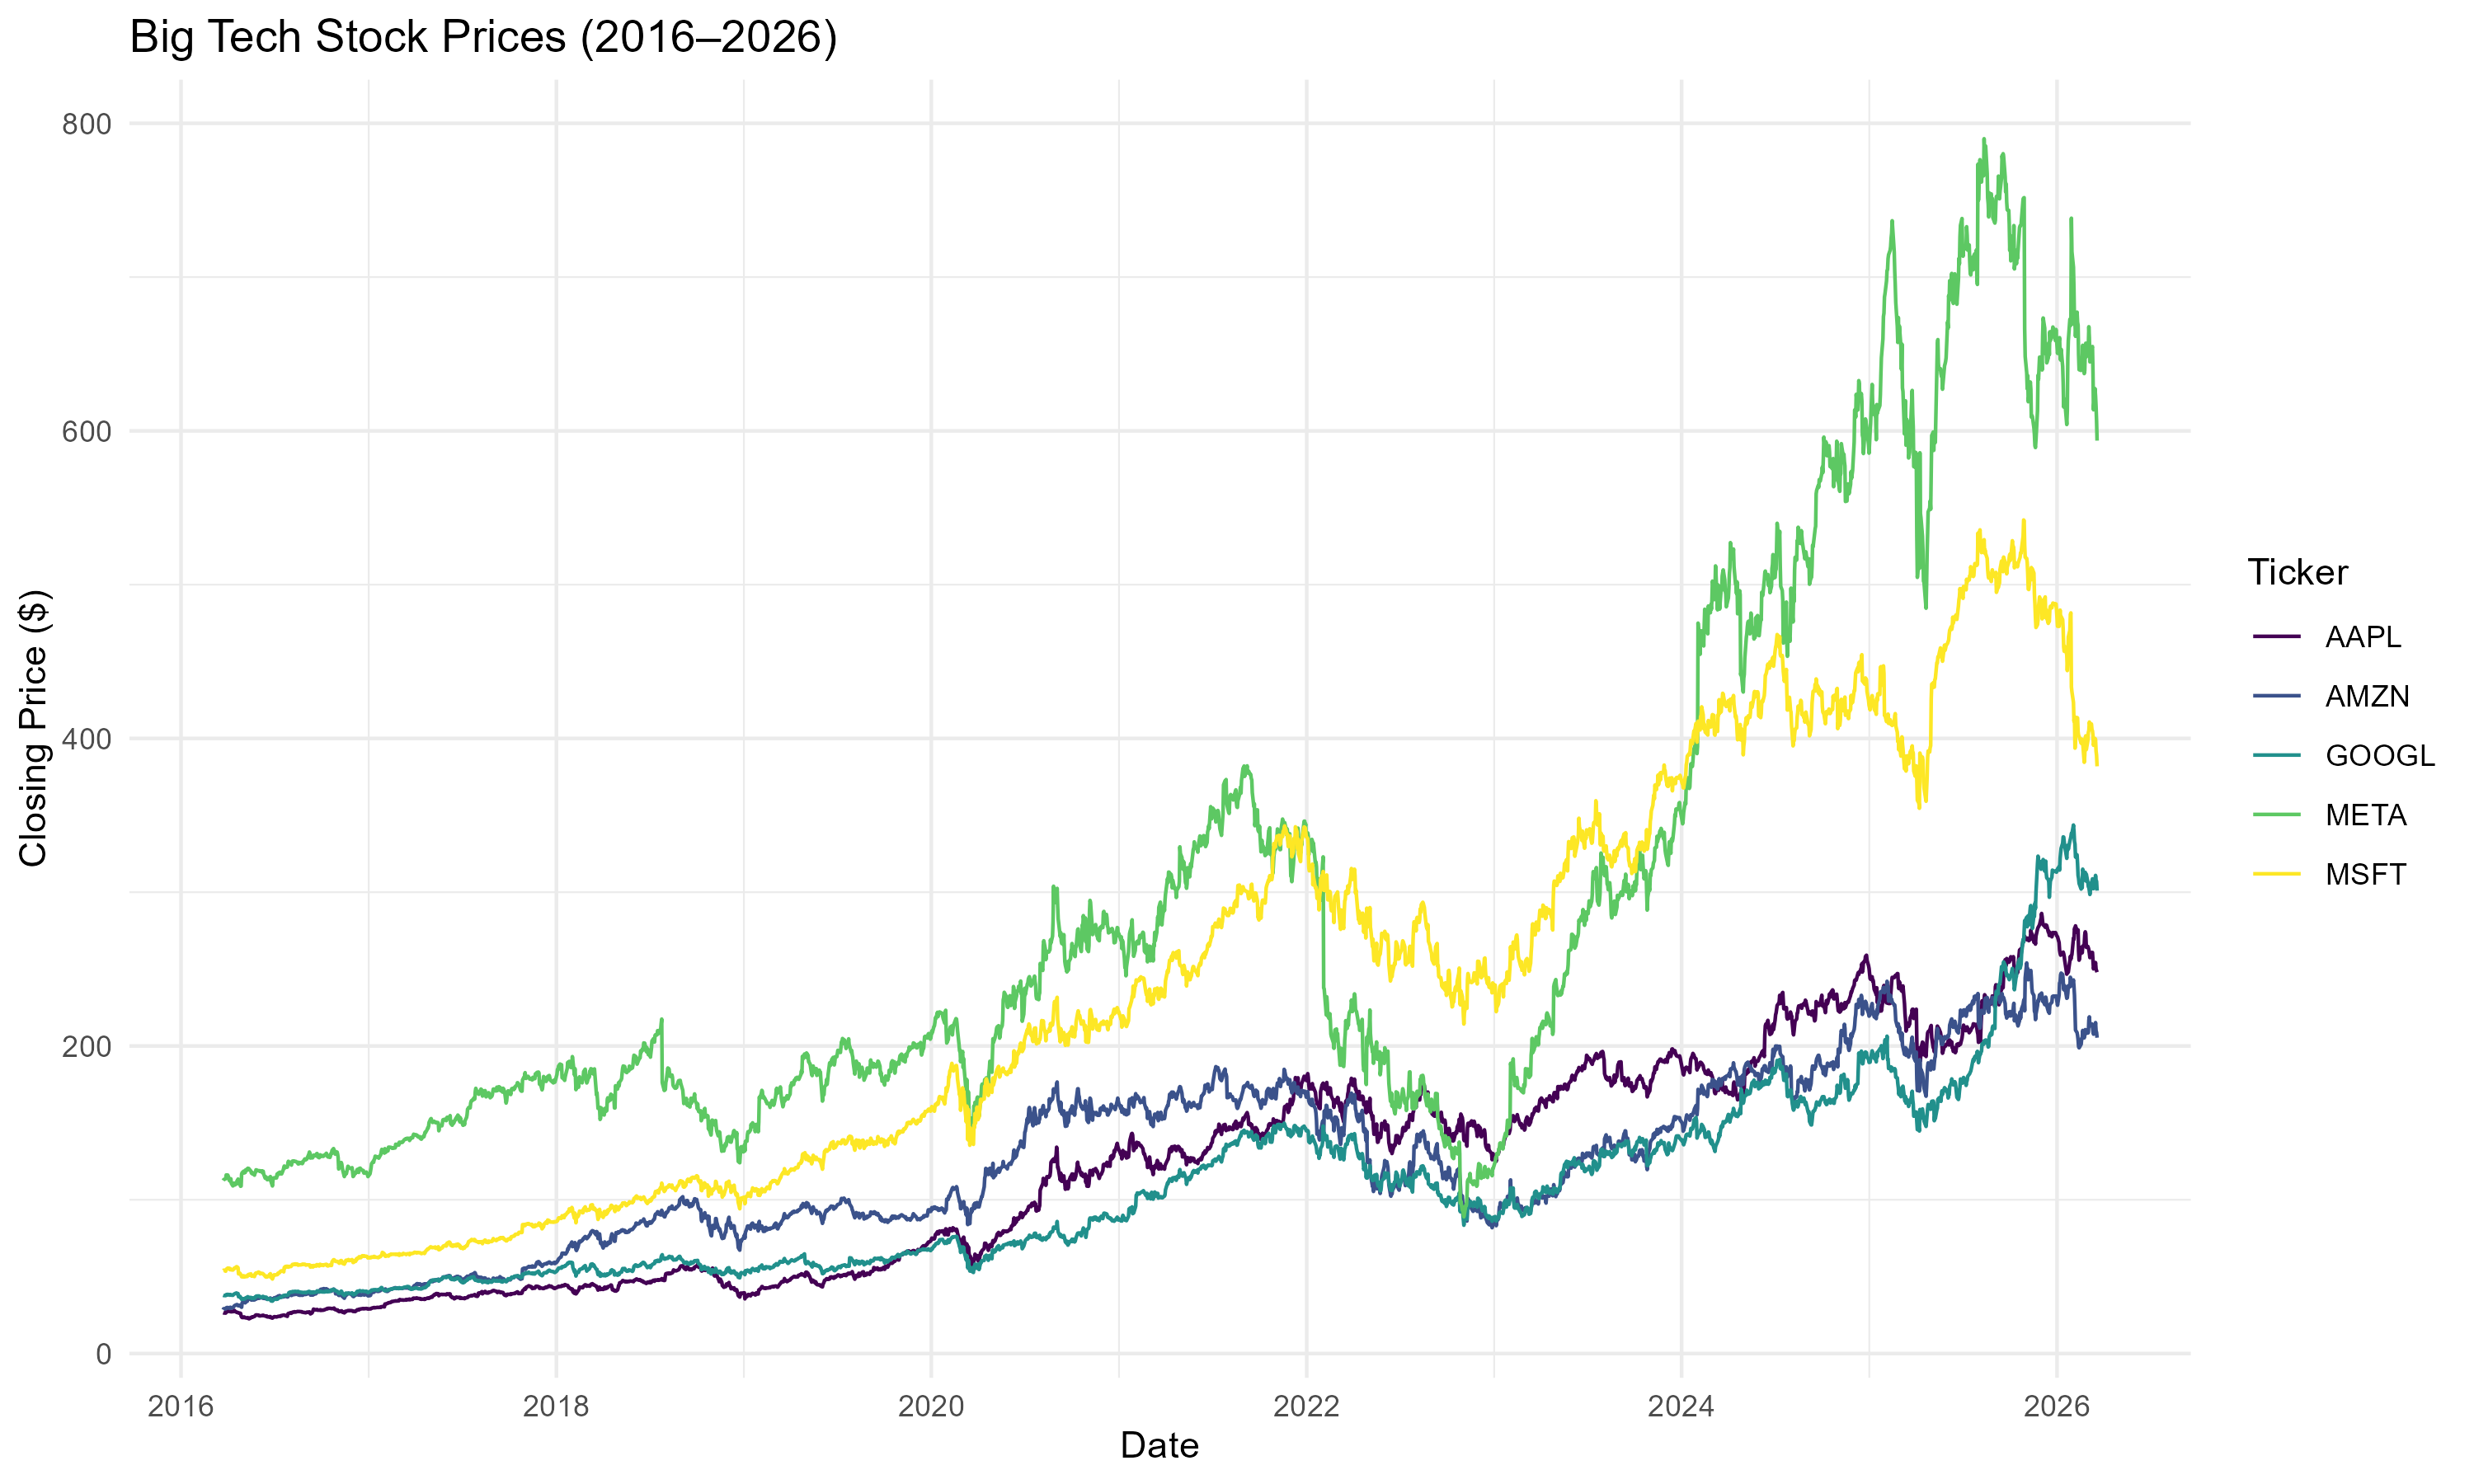
\includegraphics[width=\textwidth]{PS6a_Myers.png}
    \caption{Closing prices for five Big Tech stocks over the past decade.}
\end{figure}

This line chart shows the closing price trajectory for all five stocks over the 10-year period. It reveals that META and MSFT experienced the most dramatic price appreciation, particularly from 2023 onward during the AI-driven rally. All five stocks show a notable dip in 2022, consistent with the broader tech selloff driven by rising interest rates. The chart also captures the early 2026 pullback in tech stocks.

\section*{Visualization 2: AAPL Close Price vs.\ 50-Day Moving Average}
\begin{figure}[H]
    \centering
    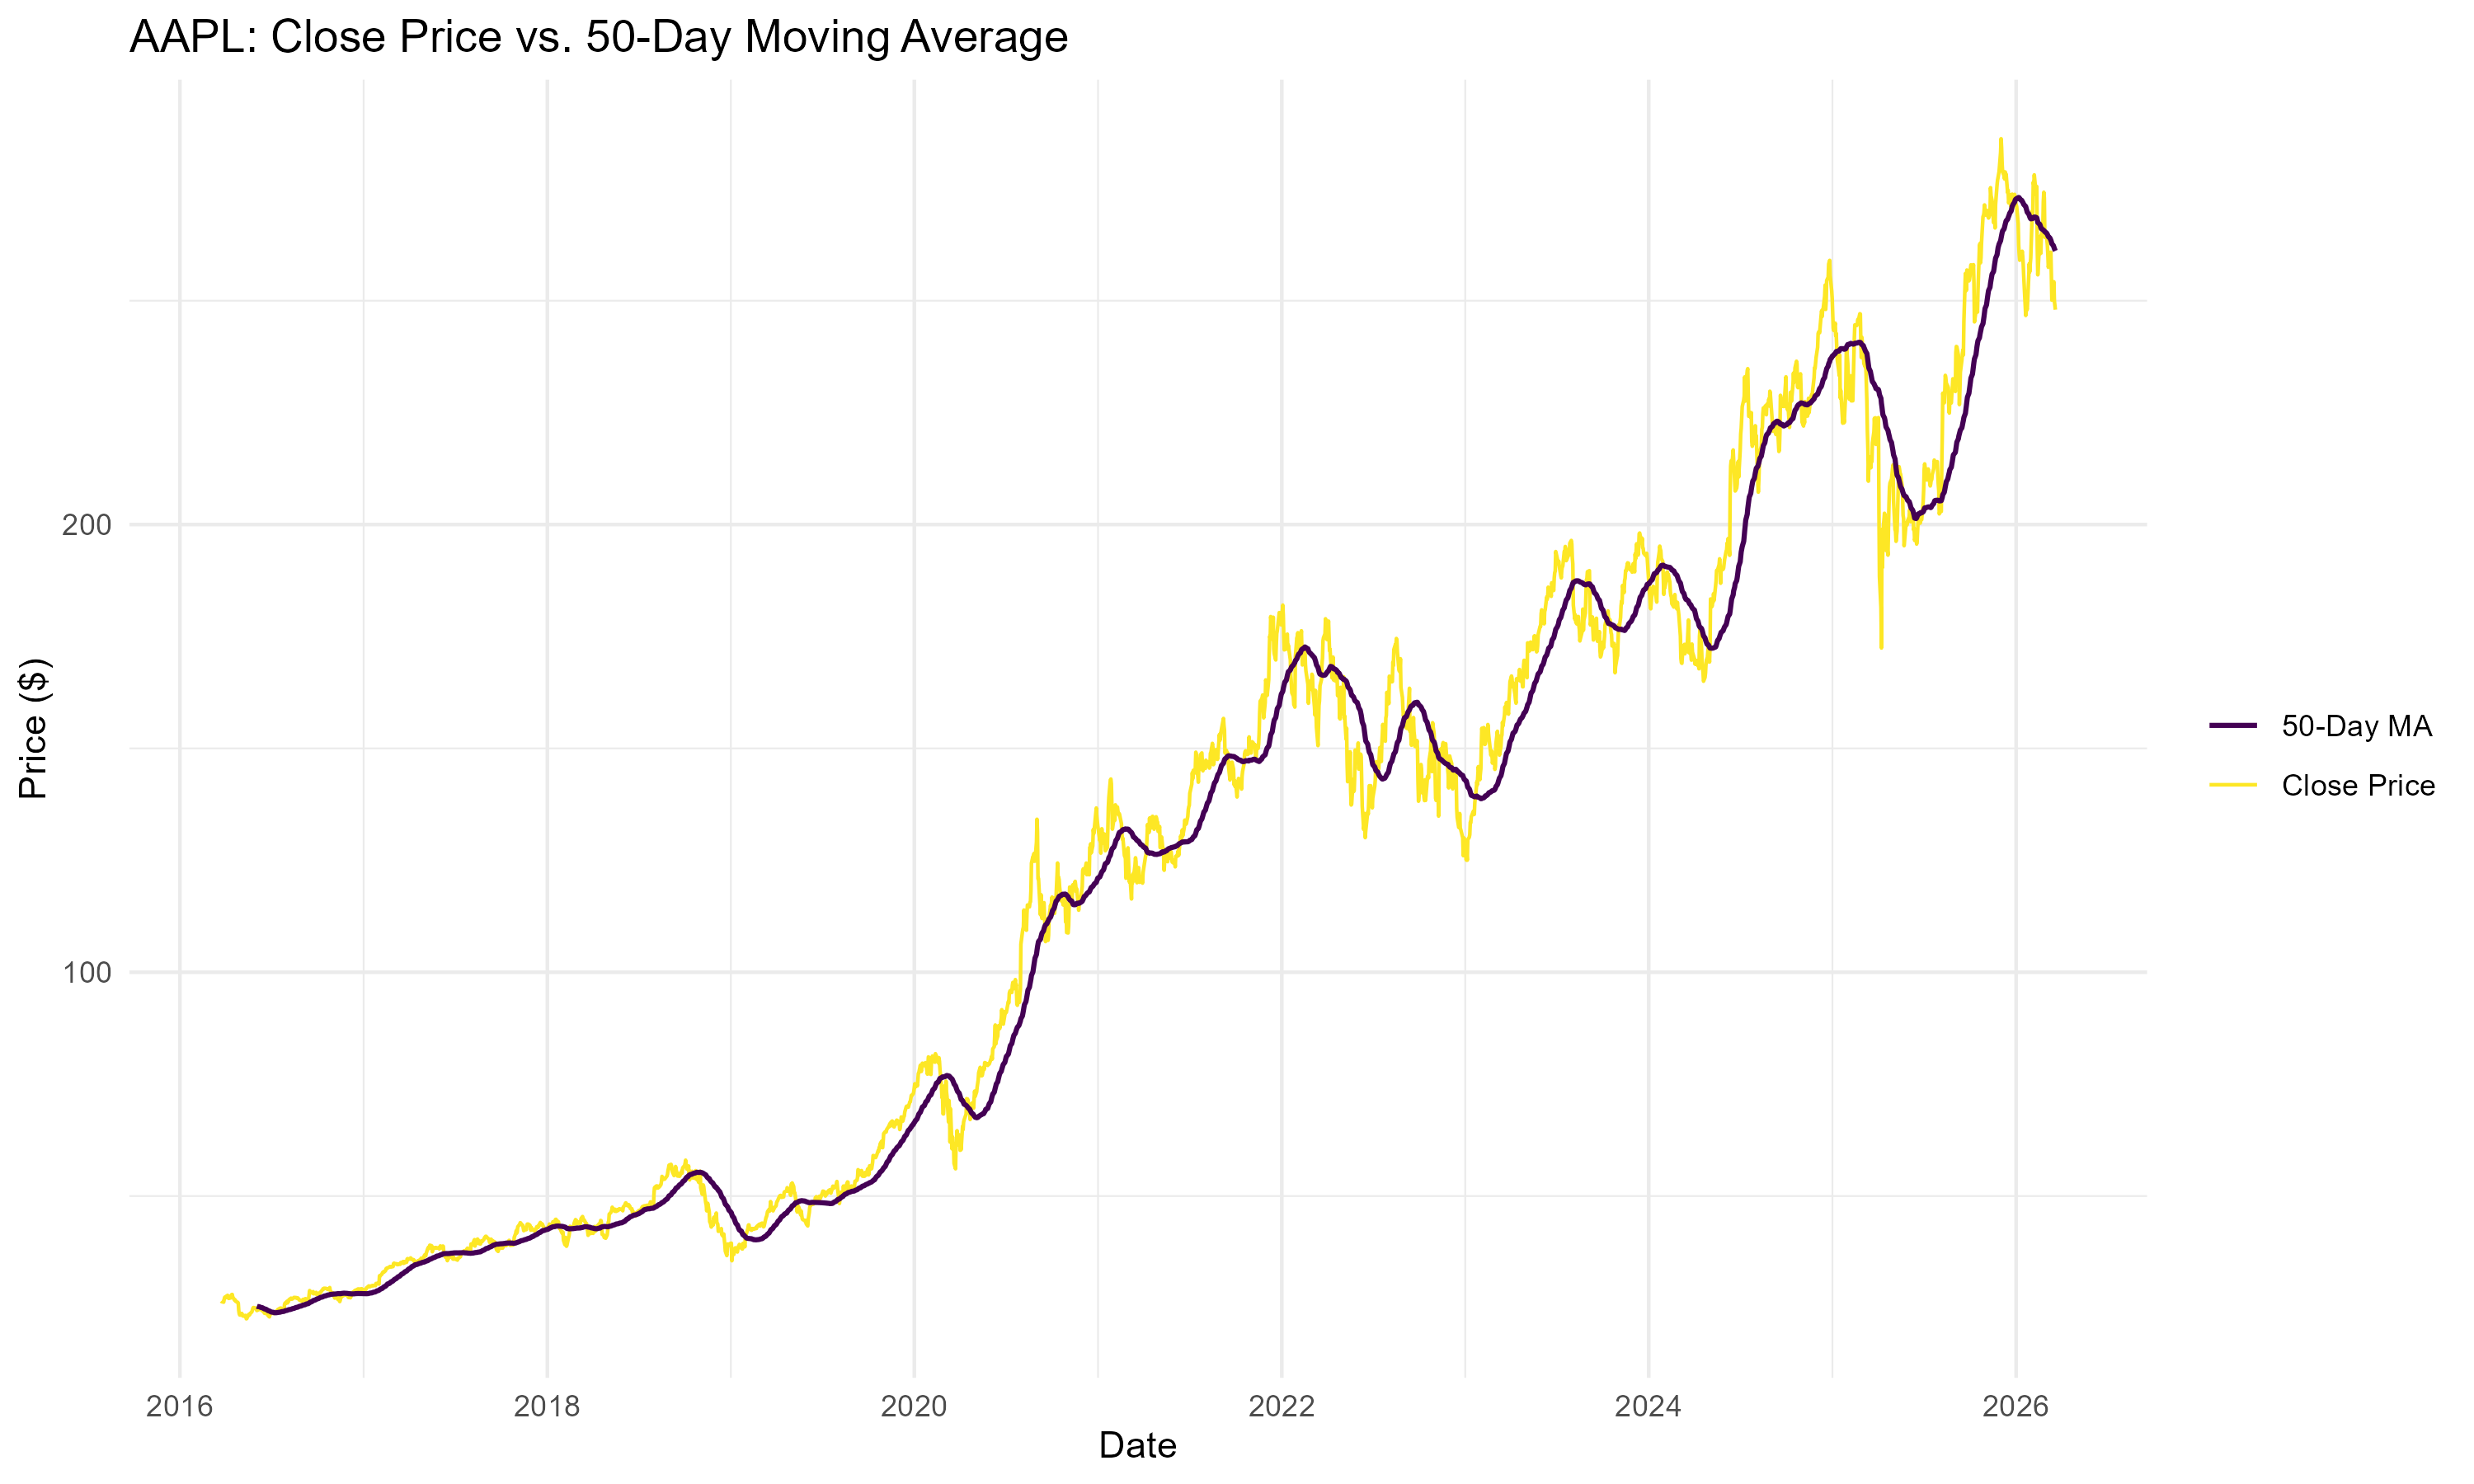
\includegraphics[width=\textwidth]{PS6b_Myers.png}
    \caption{Apple's daily closing price compared to its 50-day moving average.}
\end{figure}

This chart overlays Apple's daily closing price with its 50-day moving average. The moving average acts as a smoothed trend line, filtering out day-to-day noise. When the closing price crosses above the moving average, it can signal upward momentum, and vice versa. This visualization is useful for understanding short-term volatility relative to the underlying trend, a common technique in technical analysis.

\section*{Visualization 3: Average Daily Return by Year and Stock}
\begin{figure}[H]
    \centering
    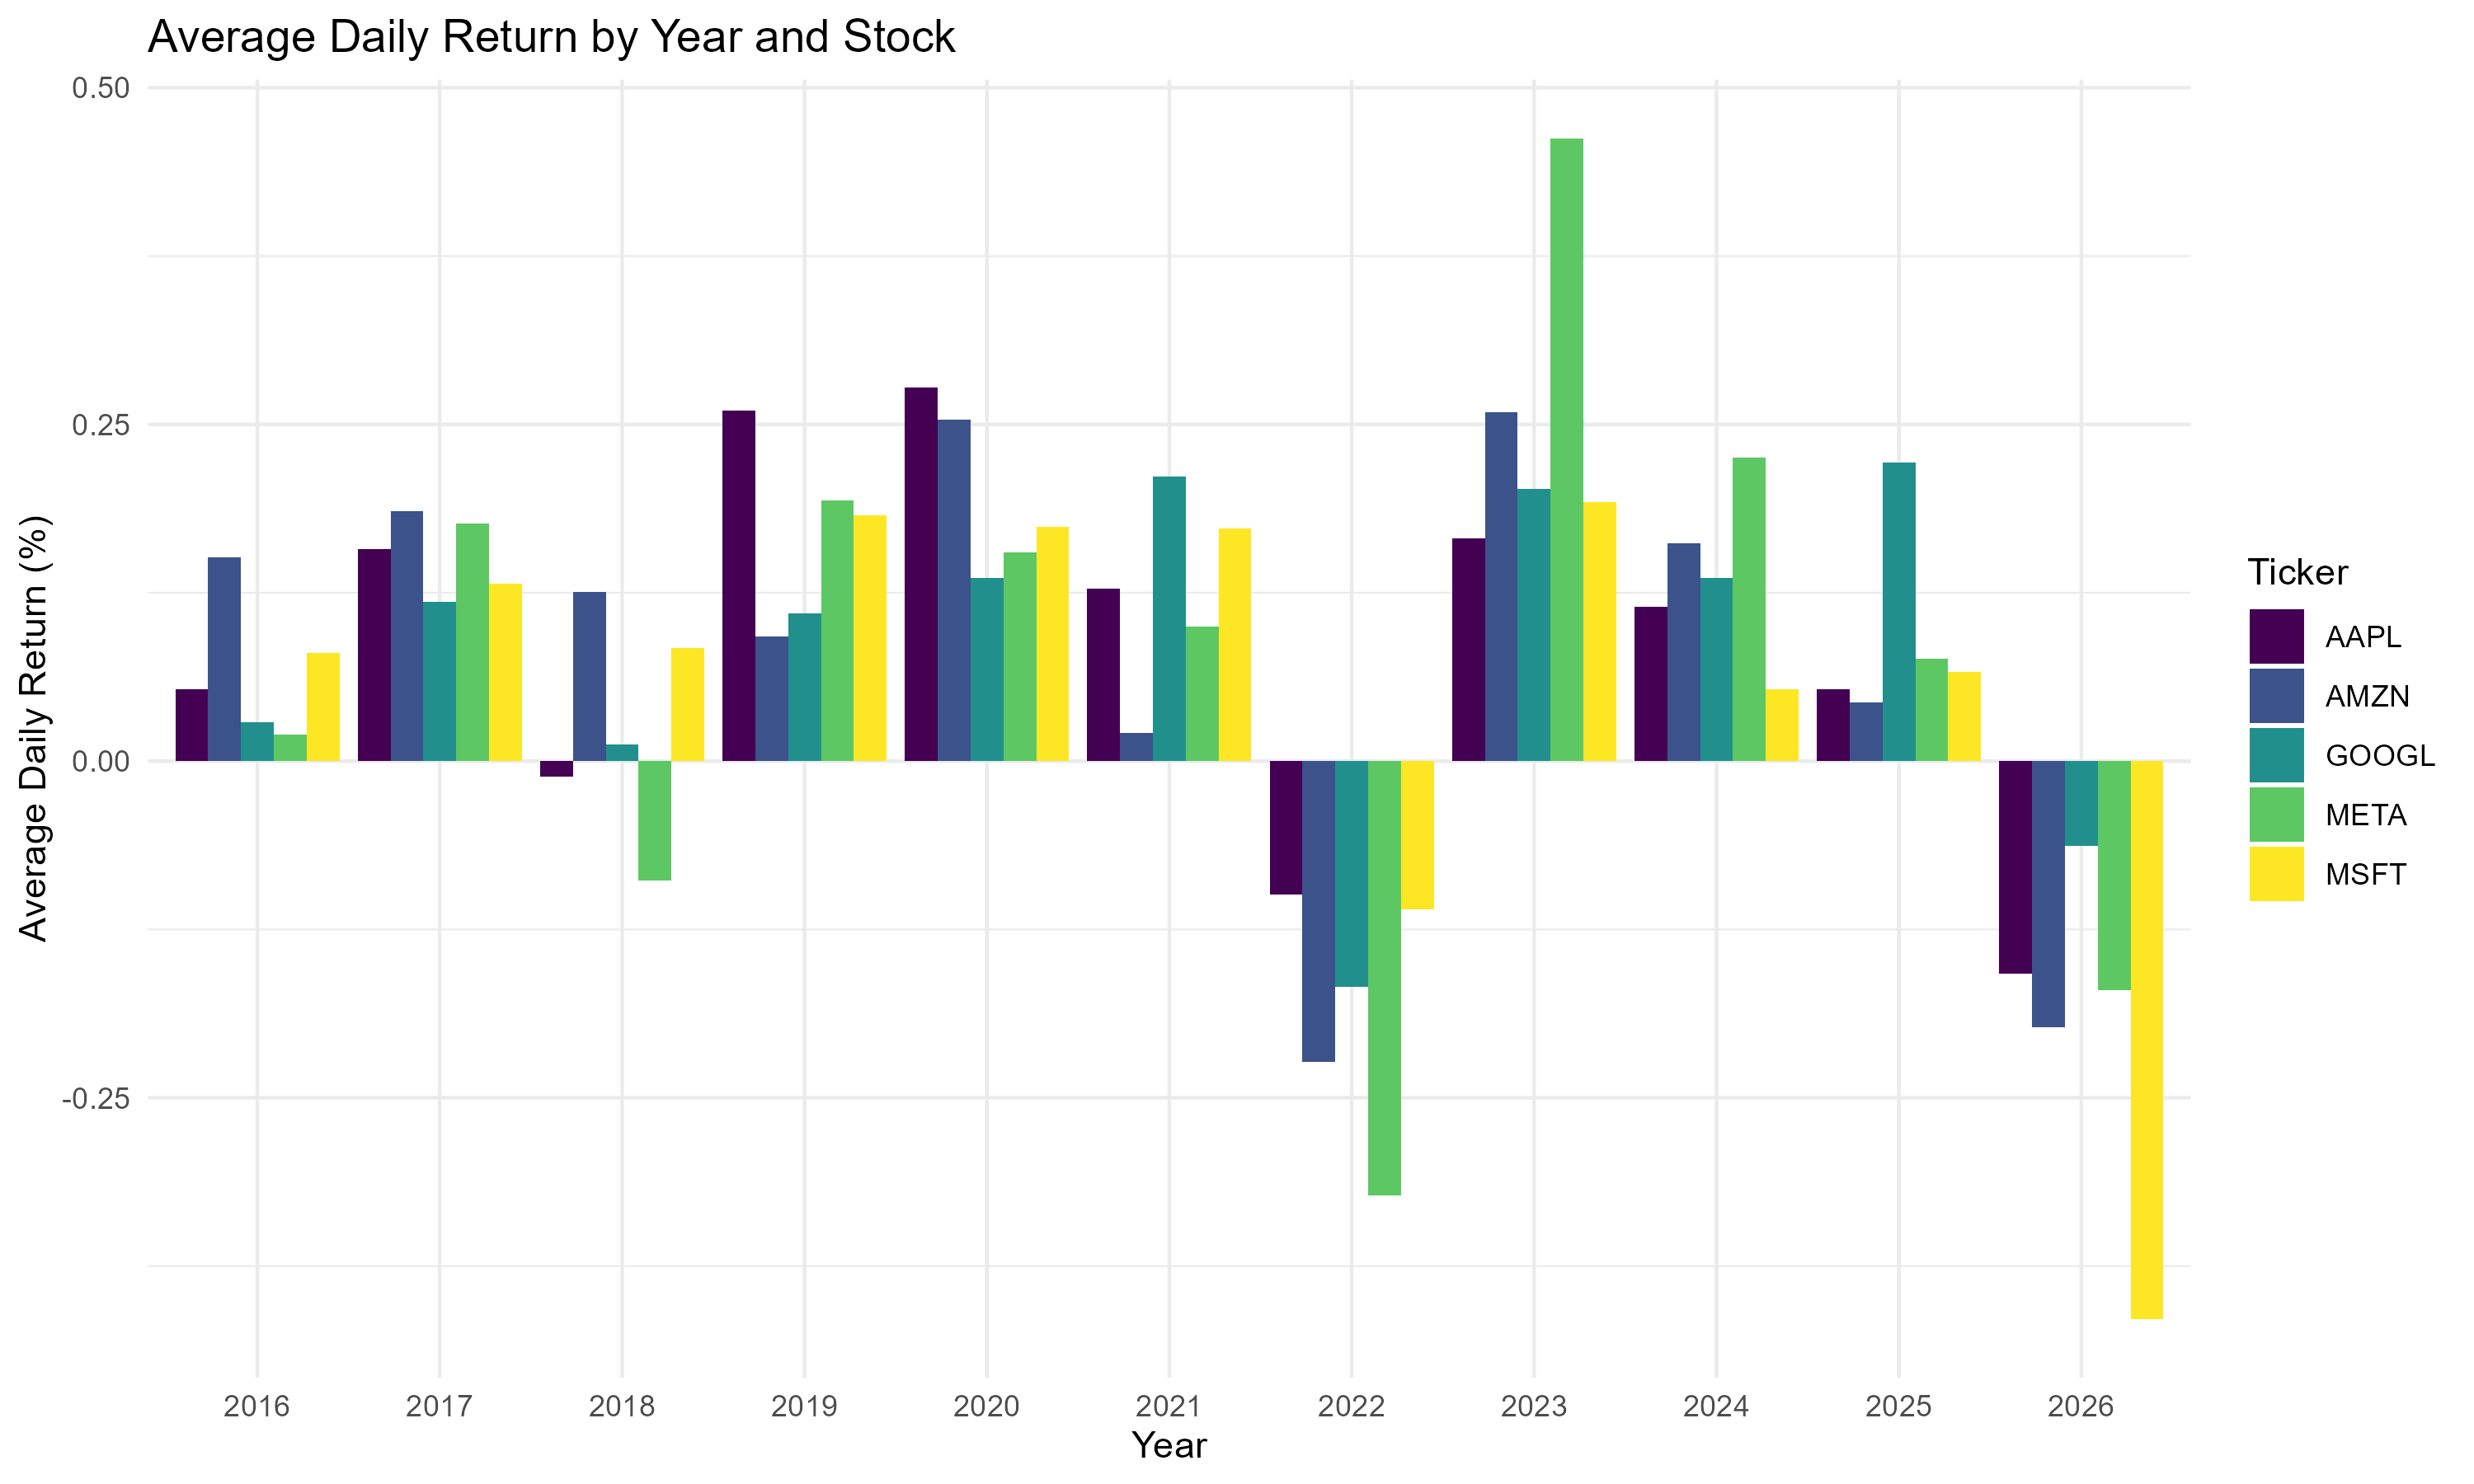
\includegraphics[width=\textwidth]{PS6c_Myers.png}
    \caption{Average daily return by year for each Big Tech stock.}
\end{figure}

This grouped bar chart shows the average daily return for each stock by year. It highlights that 2022 was a broadly negative year for Big Tech, with META experiencing the largest losses. In contrast, 2023 saw a strong rebound, especially for META. The 2026 bars (partial year) show negative returns for most stocks, consistent with the recent tech sector downturn. All three visualizations use a colorblind-friendly viridis color palette.

\end{document}